\section{Method}
Prerequisite to testing the tools is installing the tools. Taffo depends on LLVM 14 or 15 to run, and is at the time of writing not compatible with newer versions of llvm (the most recent version is 20). To install LLVM 15 you can build it from the source code following the instructions found at llvm.org, otherwise you may pull a pre-built binary. To install the pre-built binaries you can use apt, but you may need to add the llvm repository for this to work. 

Building Taffo was only successful when using pre-built binaries. 
The other tool that was used was floatsmith. This can be installed the easiest using their provided docker image, and mounting the project you want to perform experiments on.

\subsection{bitwise fault injection}
Bitwise fault injection was done thorugh manually performing an xor operation in llvm IR on the values to be subjected to faults.

%example of xor operation?
\begin{figure}[h!]
    \centering
    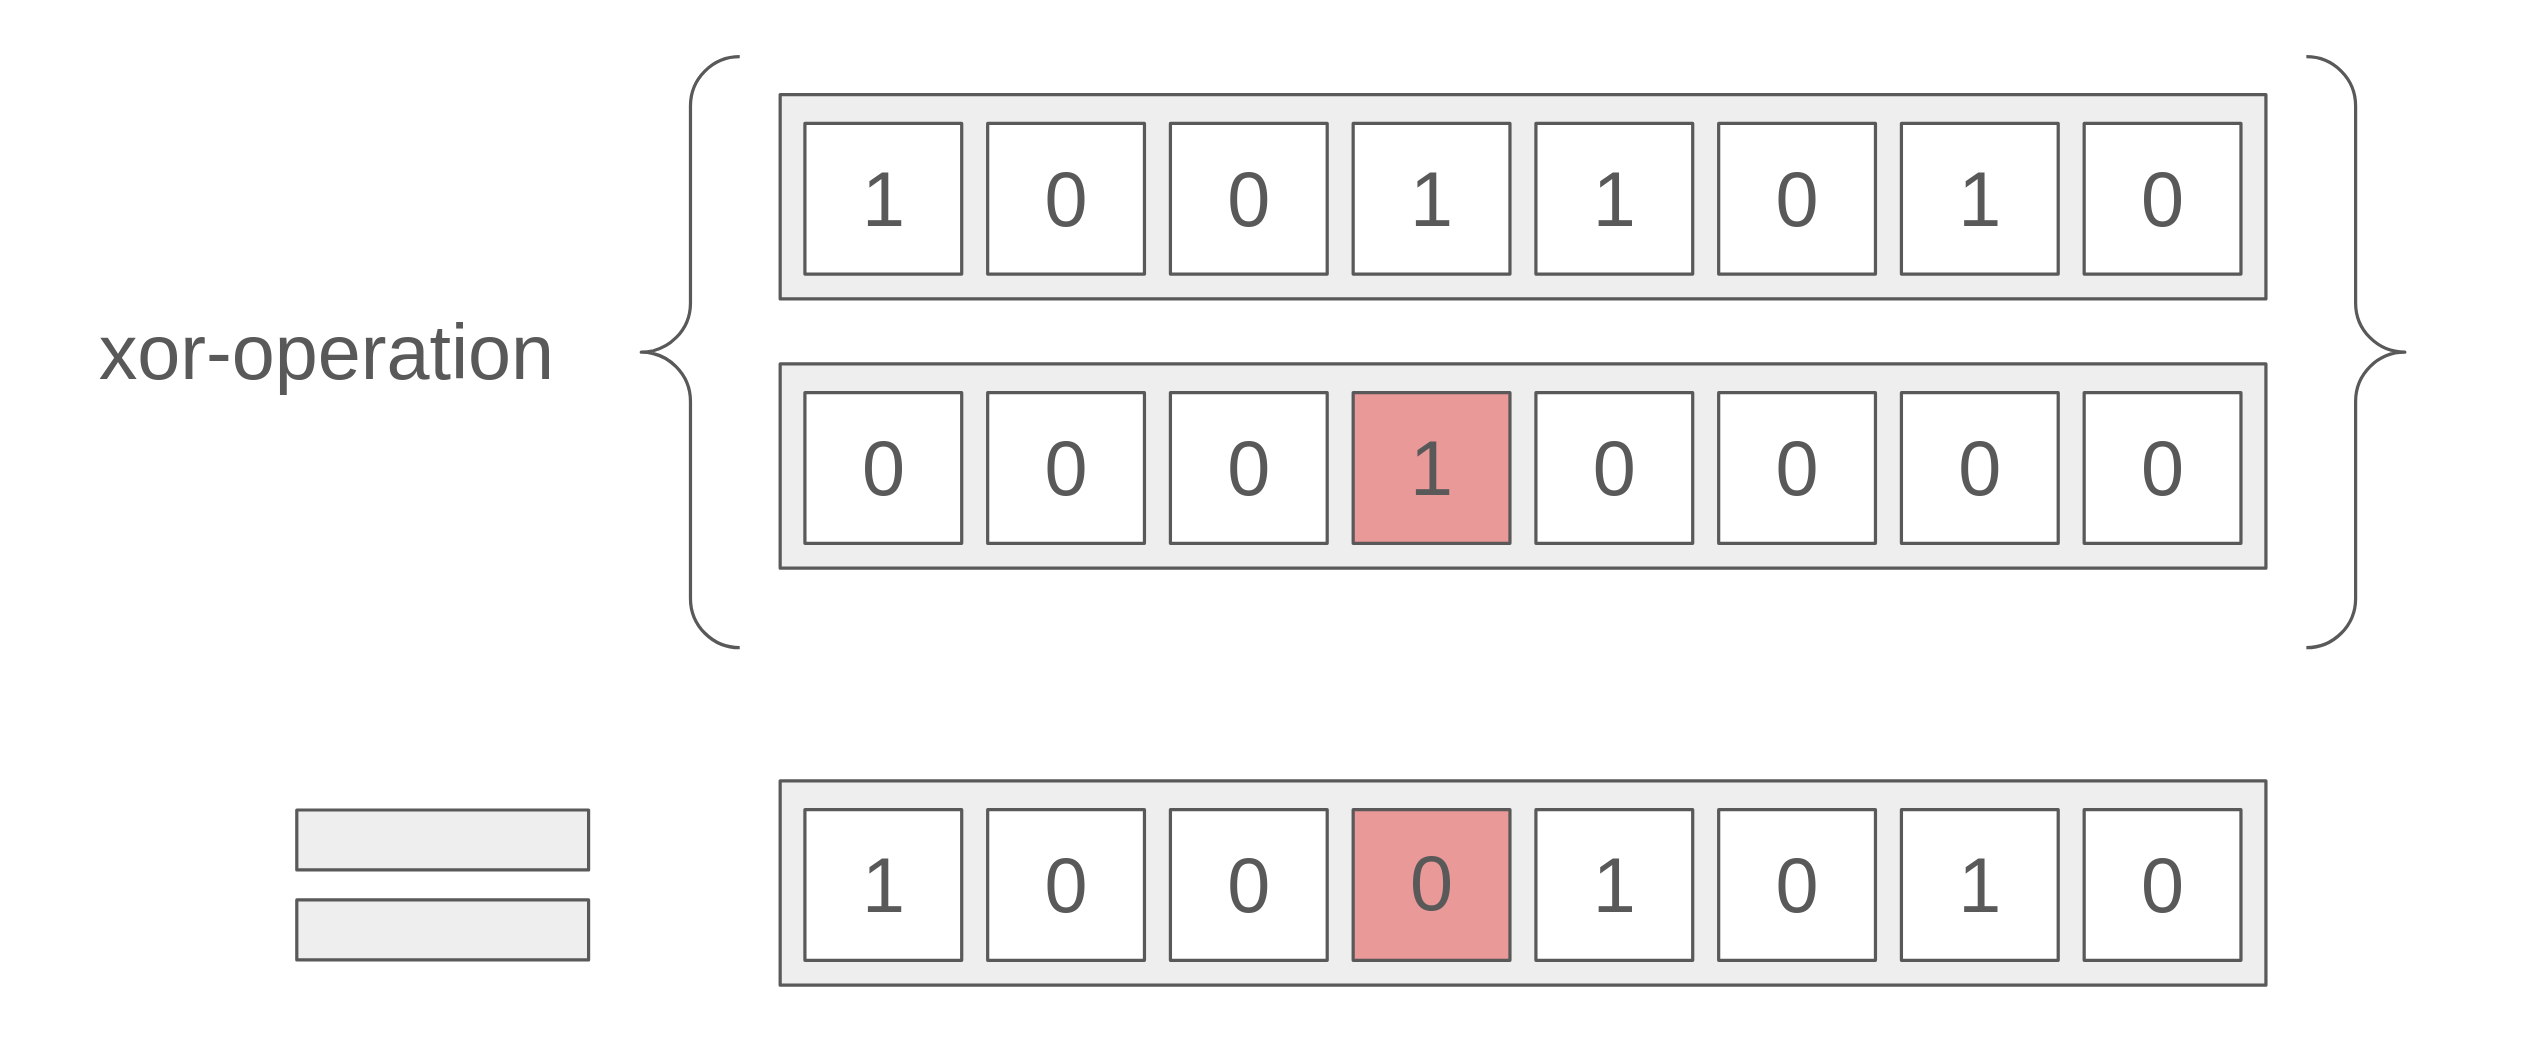
\includegraphics[width=0.5\linewidth]{Images/xor_operation.png}
    \caption{An example xor operation between two numbers. The xor operation ensures that only the operation }
    \label{fig:xor_operation}
\end{figure}

The first fault injection campaign consisted of single bit fault injections. This consisted of taking a sample benchmark from the taffo repository, compiling it to an intermediate format, in this case the LLVM IR, then flipping single bits one location at a time, and building it to a fault injected executable. For taffo, which converts floating point values to lower precision fixed point values, this requires creating a fault injected version for both the fixed and floating point intermediate format.

For each pair of fault injected executables, the outputs are compared between each other and the original floating point implementation.

To streamline injections, a helper script was created based on the existing scripts in the TAFFO repository. This allows a user to compile the selected benchmark from a list of benchmarks to llvm IR, inject faults in a user-selected location in the code, then change the bit location of this fault, and compile many different versions of the same benchmark with different faults injected in the same location. The script then runs all the benchmarks and collects output. Finally a python script that reads these outputs collects and compares them in a human readable format.

The scripts are rather ad-hoc and requires some editing of code depending on the amount of bits that the user of the scripts wants to flip for one location.

The comparison script written in python was written in a separate repository with tests, and simply copied over. This process would have benefitted from some kind of streamlining as well. 

\section{AI use}
AI was for the most part not used in neither the report nor the project part of the thesis, save for one instance. During a period of very slow progression, there was an attempt to coerce chatGPT to make sense of the build errors given by taffo when trying to build it using clang15 built from source in debug mode. This led to many answers, though unfortunately no good ones. This only served to reinforce my opinion that relying on large language models for anything is a net waste of time. 
